\documentclass[conference]{IEEEtran}
\IEEEoverridecommandlockouts
% The preceding line is only needed to identify funding in the first footnote. If that is unneeded, please comment it out.
\usepackage{cite}
\usepackage{amsmath,amssymb,amsfonts}
\usepackage{algorithmic}
\usepackage{graphicx}
\usepackage{textcomp}
\usepackage{xcolor}
\def\BibTeX{{\rm B\kern-.05em{\sc i\kern-.025em b}\kern-.08em
    T\kern-.1667em\lower.7ex\hbox{E}\kern-.125emX}}
\begin{document}

\title{COMP9517 Computer Vision Individual Project}

\author{\IEEEauthorblockN{ Siyu Gao}
\IEEEauthorblockA{\textit{z5243425} \\ \textit{University of New South Wales} }
}

\maketitle

\begin{abstract}
In this project, a number of methods for extracting leaf data characteristics were compared and used with different classifiers to identify and predict. With horizontally comparasion as well as analysis on accuracy and other metrics of each model.
\end{abstract}

\begin{IEEEkeywords}
plant image, segmentation, classification, feature extraction
\end{IEEEkeywords}

\section{Introduction and Background}
With the development and progress of human civilization, the mode of getting along with nature requires deeper development. For plants, the study of their biological characteristics, growth patterns and maturity must first be based on the correct classification. For this purpose, this project has performed the basic classification task of tobacco and Arabidopsis. First of all, the data comes from the website www.plant-phenotyping.org/. This project selected all tobacco and Arabidopsis RGB format pictures and corresponding labels in its plant file directory. There are 165 sets of Arabidopsis data and tobacco data. 62 groups. 

\section{Method (implementation)}

\subsection{Analyze the given topic}

After analyzing the given topic, the basic project framework has been divided into three major parts: the first step is to preprocess the data image, the second step is to perform feature extraction on the processed image and then the data set segmentation, and the third Step by step model establishment, classification and prediction, and finally analyze and summarize the prediction results.

\subsection{Preprocessing}
\subsubsection{Color format of image}
 
 Images acquired in a natural environment are easily affected by natural lighting, occlusion, and shadows, that is, they are more sensitive to brightness. In monochrome, the human eye is the least sensitive to red and the most sensitive to blue, so the RGB color space is a color space with poor uniformity. 
the HSV color space is used more in image processing, closer to people's experience of color perception than RGB. It is very intuitive to express the hue, vividness and brightness of the color, which is convenient for color contrast. In HSV color space, it is easier to track objects of a certain color than BGR, and it is often used to segment objects of specified color.

\subsubsection{Size of image}
\begin{figure}[htbp]
\centerline{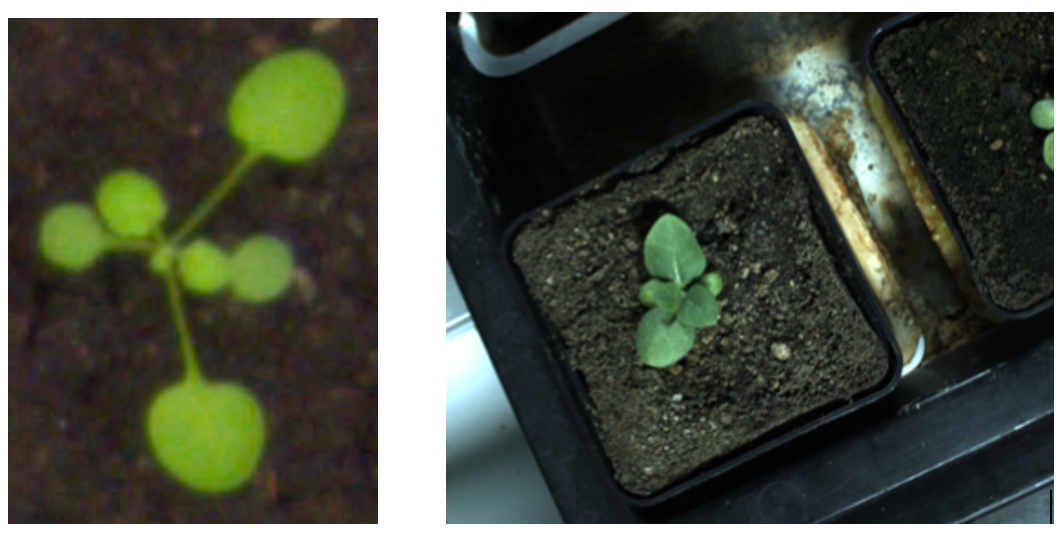
\includegraphics[scale=0.4]{p2.png}}
\caption{it is found that the size of the image files in the Arabidopsis class are different, and the size is about 100*100, but the images of tobacco leaves are all maintained at the size of 2448*2048.}
\label{fig2}
\end{figure}

By observing the size of the two types of pictures(Figure 1  are exapmles given from datasets.) 
Because the picture vectors obtained by pictures of different sizes may have large differences, resulting in classification over-fitting. Considering that the actually classified plants in the picture occupies one-tenth of the area of the picture, it cannot be purely The picture is cut, so it is necessary to adjust the size of all pictures uniformly. 
Figure 1  are exapmles given from datasets.



\subsection{Feature extraction}\label{AA}
There are usually many image features that can be used to classify plant leaves, such as shape features, color features, and texture features. In this project, the main purpose is to correctly identify the types of Arabidopsis and tobacco. Therefore, the governor of a single leaf, Commonly used absolute value features such as area, vertical axis length, and horizontal axis length are not suitable for classification basis. In this project, three methods including SIFT, SURF and HOG were used for feature extraction.

\subsubsection{SIFT and SURF}
In computer vision, the introduction of scale-invariant features, the main idea is that each detected feature point is accompanied by a corresponding size factor. When we want to match different images, we often encounter the problem of different image scales. The distance between the feature points in different images becomes different, and the object becomes different sizes. The SURF algorithm is similar to the SIFT algorithm. The SIFT algorithm is more stable and has more feature points, but the complexity is higher, while the SURF has simple calculations, higher efficiency, and shorter calculation time.
\begin{itemize}
\item Constructing Hessian matrix to construct Gaussian pyramid scale space.
\item Using non-maximum suppression to initially determine feature points.
\item Pinpoint extreme points.
\item Select the main direction of the feature point.
\item Construct a description operator for surf feature points.
\end{itemize}

\subsubsection{HOG}
In an image, the Histogram of Oriented Gradient (HOG) can well describe the features of the local target area and is a commonly used feature extraction method.
\begin{itemize}
\item Calculate the gradient of each pixel of the image (including size and direction), and capture contour information;
\item Combine 4 cells to form a block (take 22 as an example), and concatenate the features of 4 cells in a block to obtain the HOG feature descriptor of the block;
\item Connect the HOG feature descriptors of all blocks in the image to obtain the HOG feature descriptor of the image, which is the feature vector of the final classification.
\end{itemize}

\subsection{Classifications}
This project has conducted experiments on the following classifiers and selected an optimal choice. For specific parameters, please refer to Section III:
\subsubsection{Support vector machines (SVM)}
SVM is a supervisable machine learning algorithm that can be used for classification and regression. Each data item is drawn in an n-dimensional space (n is the number of features of each data point), and the classification is done by finding the best hyperplane to distinguish between the two classes. 

\subsubsection{K-Nearest Neighbours (KNN)}
By searching for the K most similar instances (neighbors) in the entire training set and summarizing the output variables of these K instances, new data points can be predicted. For digital data sets, it is possibel to directly use the Euclidean distance metric. This is defined as the square root of the sum of squared differences between two numeric arrays.
\subsubsection{Random Forest Classifier (RF)}
The RF classifier consists of several independent decision trees, which operate as a whole. Each individual decision tree performs category prediction, and the category with the highest number of votes becomes the model prediction. Many unrelated models run together to make better predictions than a single model.

\section{Experiment}
\subsection{Overall framework}
The code of this project has designed two classes, namely IMG and DATASETS.
\subsubsection{IMG Class}
In the IMG class, the following functions are implemented:
\begin{itemize}
\item Unified pictures export the matrix of different color formats and store them in the same object: 
Save them in 
IMG.original\_image, 
IMG.image\_RGB, 
IMG.image\_GRAY, 
IMG.image\_HSV.
\item Use the IMG.resize(self) function to export matrices of different sizes and store them in the same object: 
Saved in 
IMG.resized\_image\_GRAY,
IMG.resized\_image\_RGB, 
IMG.resized\_image\_GRAY, 
IMG.resized\_image\_HSV.
\item Generate the Watershed segmentatation picture and 
Meanshift segmentatation picture corresponding to the picture function, and package them in the object.
\item The built-in function automatically generates the corresponding feature sequence of 
the image after obtaining the image matrix according to different feature extractors, 
using 
IMG.get\_surf(self), 
IMG.get\_sift(self), 
IMG.get\_hog(self)
, etc. 
The acquired image features are stored in 
IMG.descriptors.
\item Decompress the feature sequence in the picture and store it in 
IMG.unzipped\_features.
\item Store the actual classification label corresponding to the picture in 
IMG.label.
\end{itemize}
\subsubsection{DATASETS Class}
In the DATASETS class, the following functions are implemented:
\begin{itemize}
\item The input value of the generated DATASETS class is the ratio of the test data set to all the data, the default is 0.25
\item Implementing DATASETS.get\_all\_imgs(self) to automatically read all the given picture data that meets the conditions, and claim an entire dictionary, where the key is the IMG object of the picture and the value is its corresponding label ( Represents whether the plant is Arabidopsis or tobacco)
\item Through the get\_datasets(self), train\_test\_split function, the complete data set obtained above is split into the training data set, the test data sets, and the training data The individual objects in the IMG object sequence of the set and the test data set are replaced with their corresponding feature data and rearranged.
\item Obtain the given classification number of all feature data through external input. This project uses Kmeans for data feature classification, and finally packs the complete training feature and test feature data in the DATASETS class.
\end{itemize}
\subsubsection{Model Class}
To build the model, train the model and model prediction:
\begin{itemize}
\item This project established three models (SVM, KNN, RF), using LinearSVC, KNeighborsClassifier, and RandomForestClassifier three classifiers respectively, and carried out data input and prediction on them respectively.
\item Use the metrics module in sklearn to compare the accuracy, precision, and average-recall percentage of the classification results.
\end{itemize}

\subsection{Experimental setup}
\subsubsection{Metrics with different fomation}
Regarding the impact of different image formats on the classifier, Table 1 shows part of the data. Obviously HSV format can bring higher accuracy, but the accuracy and recall rate of 1 is very eye-catching. Further analysis, it is obvious that considering the comprehensive consideration of time and space complexity and final classification accuracy, grayscale format and unclassified image format should be discarded, and subsequent experiments will continue to retain RGB and HSV formats.
\begin{table}[htbp]
\caption{Metrics with different fomation of image input}
\begin{center}
\begin{tabular}{|c|c|c|c|c|c|}

\hline
image fromat& Resize &Acc&Rec &Roc&Time(s)\\
\hline
RGB& Y&0.913043&0.842105  &0.842105&48\\
\hline
RGB& N&0.985507 &0.973684  &0.973684&12\\
\hline
HSV& Y&1.000000&1.000000 &1.000000&50\\
\hline
HSV& N&0.985507&0.990000 &0.990000&10\\
\hline
GRAY& Y&0.956522 &0.921053  &0.921053&40\\
\hline
GRAY& N&0.971014 &0.963684  &0.963684&9\\
\hline

\end{tabular}
\label{tab1}
\end{center}
\end{table}

\subsubsection{Metrics with differen feature extraction method}
Table 2 shows the classification performance of RGB color pictures and HSV color pictures on the same classification model after feature extraction by three different feature extractors after rescaling. It can be found that the operating time of SIFT is 1 times longer than that of HOG and SURF, and the accuracy and other indicators have not been significantly improved.

\begin{table}[htbp]
\caption{Metrics with differen feature extraction method}
\begin{center}
\begin{tabular}{|c|c|c|c|c|c|}

\hline
extraction&format  &Acc&Rec &Roc&Time(s)\\
\hline
SIFT& RGB&0.927536 &0.868421   &0.868421 &80\\
\hline
SIFT& HSV&0.915407  &0.901000  &0.901000&12\\
\hline
SURF& RGB&0.956522 &0.921053   &0.921053 &13\\
\hline
SURF& HSV&0.971014 &0.960973   &0.960973 &12\\
\hline
HOG& RGB&0.875310&0.852105  &0.852105&48\\
\hline
HOG& HSV&0.896514 &0.903684  &0.903684&12\\
\hline

\end{tabular}
\label{tab2}
\end{center}
\end{table}


\subsubsection{Kmeans' different K value selection}

The essence of K-means is a data partitioning algorithm based on Euclidean distance. Dimensions with large mean and variance will have a decisive impact on the clustering of data. Therefore, data that has not been normalized and united cannot be directly involved in calculations and comparisons. Common data preprocessing methods are: data normalization and data standardization.
In addition, outliers or noisy data will have a greater impact on the mean, resulting in a center shift, so we also need to detect abnormal points in the data.
The selection of K value has a great influence on K-means, which is also the biggest shortcoming of K-means. Common methods for selecting K value are: elbow method and gap statistic method.

\begin{figure}[htbp]
\centerline{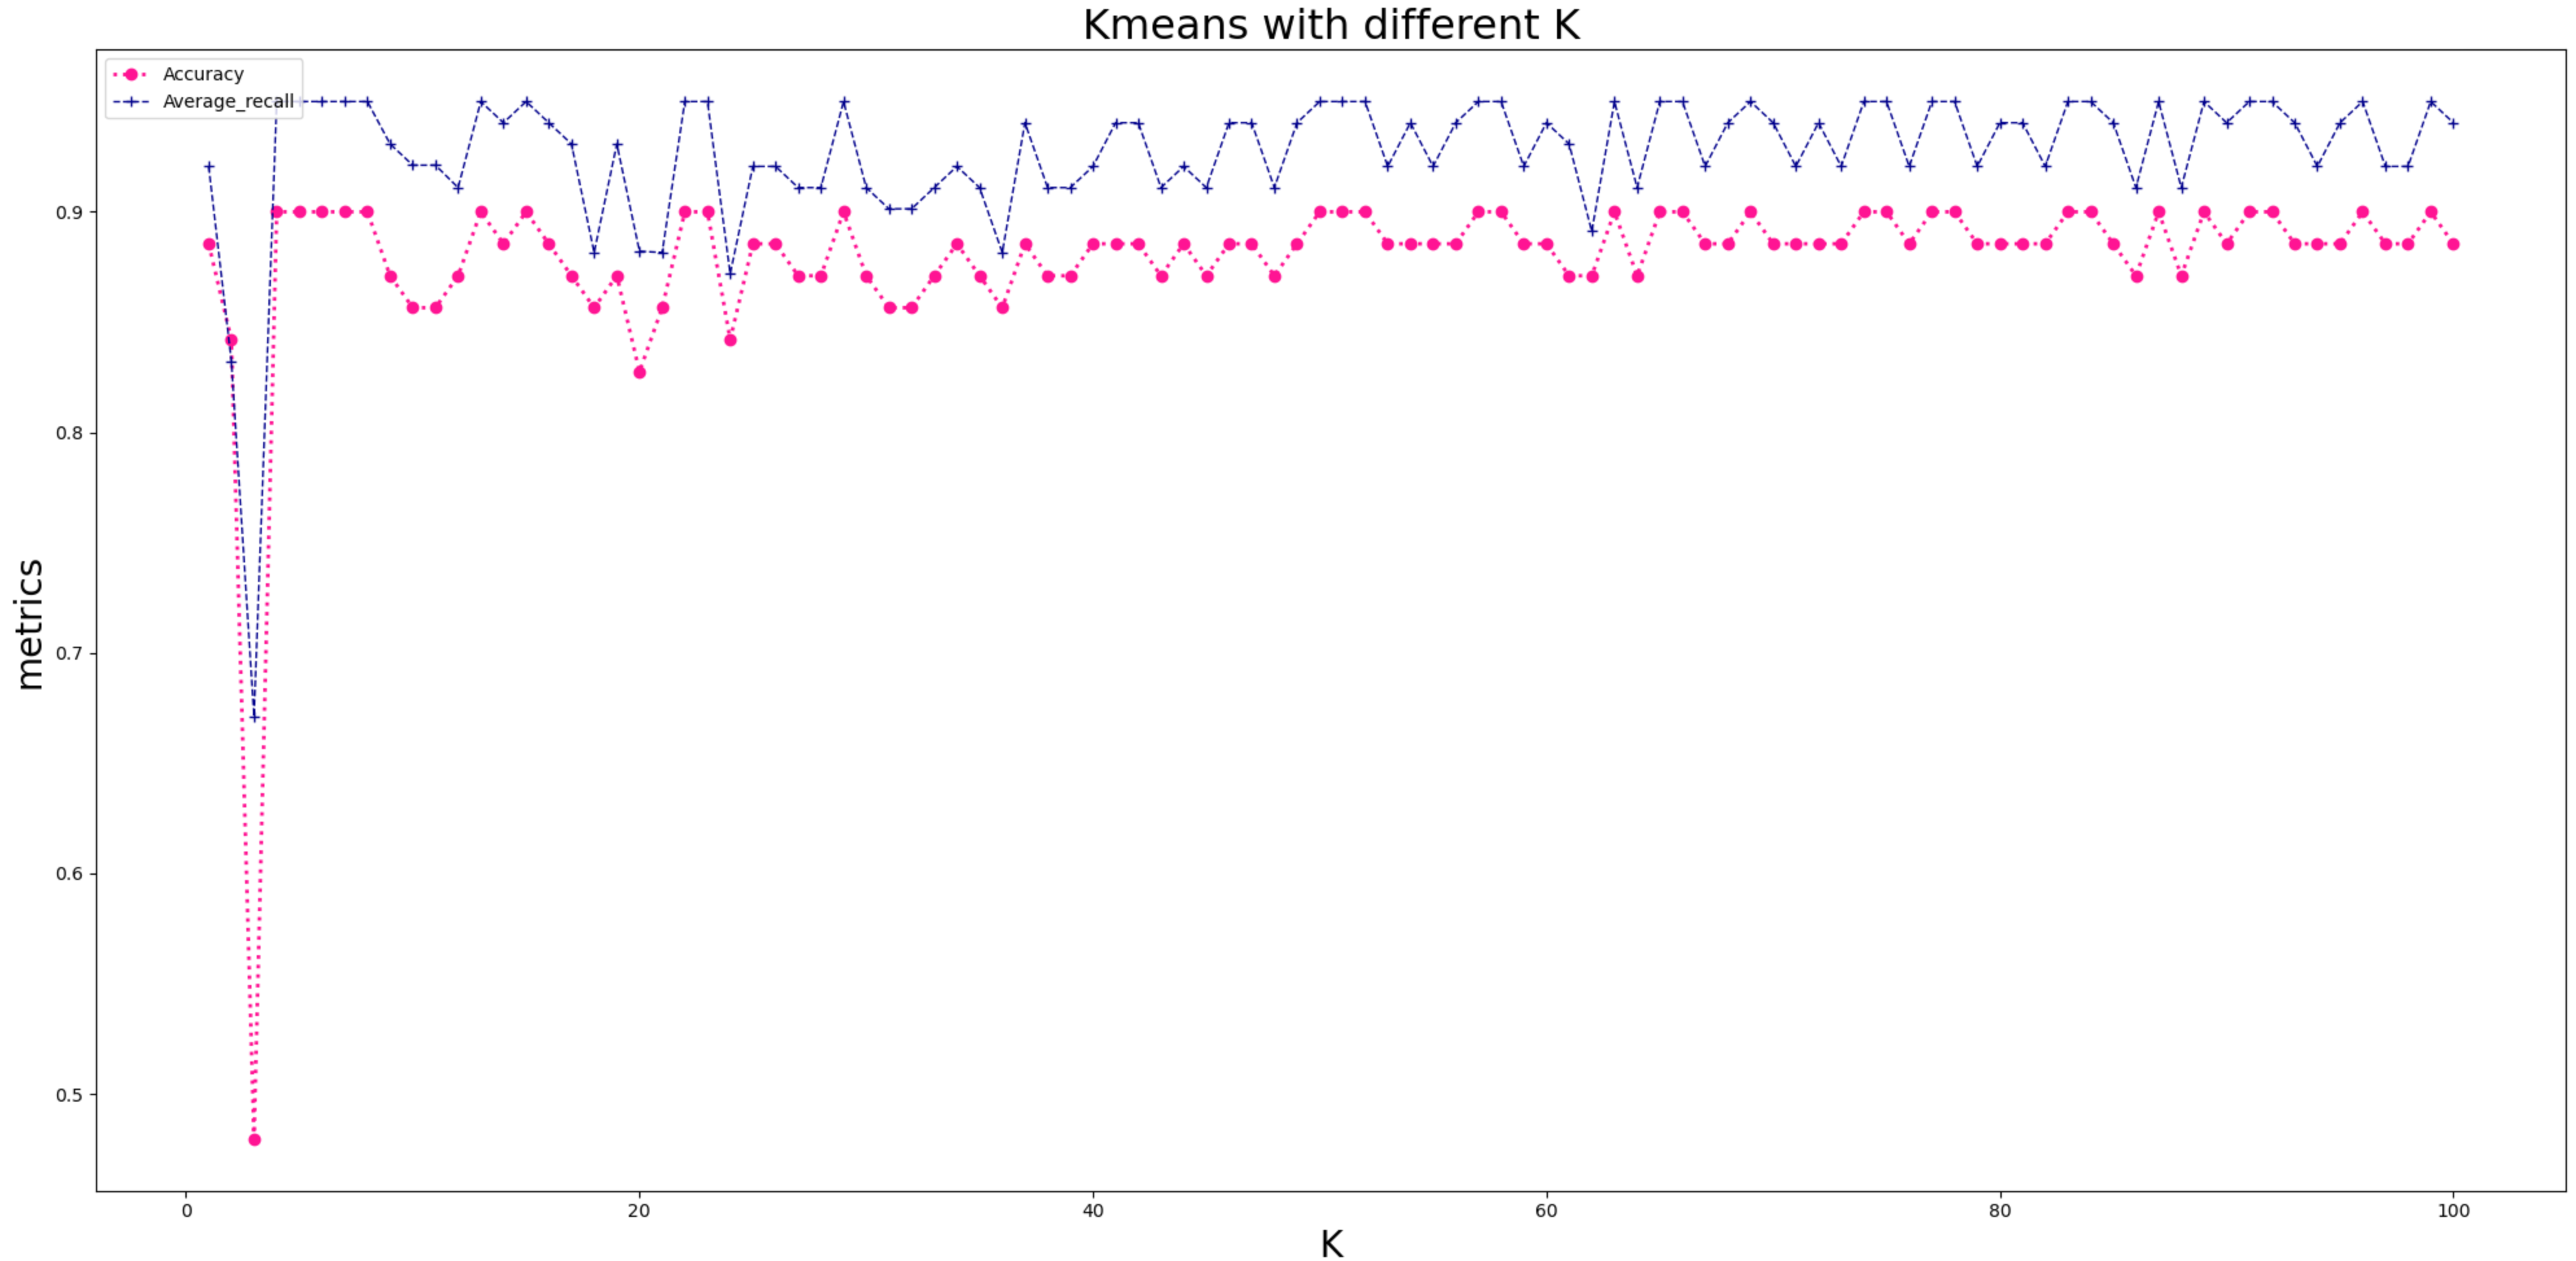
\includegraphics[scale=0.12]{p3.png}}
\caption{Comparesiton of given examples.}
\label{fig2}
\end{figure}
It can be seen from the Figure 2 that when the value of K is greater than 60, the accuracy and recall rate are obviously stable around 0.9, so any K value between 60-100 is acceptable.
\section{Results and Discussion}
First of all, in response to the problem of multiple metrics reaching 1 in this project, many documents have been referenced. At first, people were suspicious of over-fitting, but after many experiments, if the phenomenon of over-fitting occurs, all the prediction data should always be kept at 100\% accuracy, but in fact it is not. In 50 trials , There are 7 times with 100\% prediction accuracy rate. Further reference materials and review the experimental data of this project. This phenomenon is likely to be caused by the small size of the data set. Since  there are 165 sets of Arabidopsis data and tobacco data 62 sets. Another reason for the analysis should focus on the image preprocessing process. After reviewing the feature data obtained by analyzing the image by surf, it is most likely that the size of the image is not unified during the preprocessing process, resulting in the data feature vector The size and the length of the original picture are the same, and the distinction is too high, which directly leads to the loss of data segmentation.Therefore, this project adopted the KFold method to expand the data set in disguised form, and achieved some results.

Below are some metrics of all three models with HSV resized format, 
and the feature extraction with SURF, metrics are averaged with KFold methods set K at 10,test size at 0.3:

\begin{table}[htbp]
\caption{Metrics of models with K-Folds}
\begin{center}
\begin{tabular}{|c|c|c|c|}



\hline
CLF &Acc&Rec &Roc\\
\hline
SVM&0.989475 &0.992592   &0.992592 \\
\hline
KNN&0.981578 &0.987037   &0.987037 \\
\hline
RF&0.995614 &0.993322   &0.993322 \\
\hline

\end{tabular}
\label{tab3}
\end{center}
\end{table}

In this article, based on a variety of preprocessing operations, the project compares and applies multiple methods of extracting leaf data features and uses different classifiers to identify and predict. The next step will focus on how to recognize plant leaf images in complex environments and further maintain or even improve the recognition rate of the hypersphere classifier of the moving center. Under such requirements, it may be necessary to adopt image denoising, Gaussian Filters,watershed, Meanshift and other operations.


\begin{thebibliography}{00}
\bibitem{b1} Minervini M, Scharr H, Tsaftaris SA. Image analysis: the new Bottleneck in
plant phenotyping. IEEE Signal Proc Mag. 2015;32:126–31.
\bibitem{b2} Qiangqiang Z, Zhicheng W, Weidong Z, Yufei C. Contour-based plant leaf
image segmentation using visual saliency. In: Zhang Y-J, editor. Image
and graphics. Cham: Springer; 2015. p. 48–59.
\bibitem{b3} Ispiryan R, Grigoriev I, zu Castell W, Schäfner A. A segmentation procedure using colour features applied to images of Arabidopsis thaliana.
Funct Plant Biol. 2013;40:1065–75.
\bibitem{b4} Singh A, Ganapathysubramanian B, Sarkar S, Singh A. Deep learning for
plant stress phenotyping: trends and future perspectives. Trends Plant
Sci. 2018;23:883–98.
\end{thebibliography}



\end{document}
